% %%%% Benifit of reasoning about 
% \subsection{Motivation of Reasoning about Adaptivity}
% %%%% Benefit of reasoning about 
% \subsection{Motivation of Reasoning about Adaptivity}
% % 
The adaptive data analysis designed for identifying  properties for unknown populations / distributions 
through data samples is widely 
used in research and industrial areas.
% , including machine learning areas, etc.. 
When generalizing the result from data sample to the unknown populations, 
the generalization error is a key issue researchers focusing on reducing.
From existing research, the \emph{adaptivity} in the analysis plays a key role in reducing the generalization error.
In this chapter, 
I firstly introduce the  cruciality for reasoning about the \emph{adaptivity} quantity property 
for adaptive data analysis program in Section~\ref{sec:intro-motivation}.
% analyzing 
Motivated by the significance of \emph{adaptivity},
in order to analyze this \emph{adaptivity} property for the adaptive data analysis, there are 3 challenges
% problems encountered.
introduced in Section~\ref{sec:intro-exe}.
% I introduce these three problems
% and the full-spectrum analysis methodologies developed according to these problems 
Targeting to the three challenges, I introduce my full-spectrum analysis methodologies accordingly.
Concretely, the full-spectrum analysis is developed through the language formalization,
the execution-based analysis and the static-based program analysis.
%
Based on the implementation and experimental results on my full-spectrum analysis, 
% I propose three significant 
% further features can be improved 
% % in the analysis methodologies 
% in Section~\ref{sec:intro-improve}, 
% and plan to finish these improvements 
% before the final defense.
% %
% Based on the implementation and experimental results, 
I introduce three significant 
further features I designed to improve the precision of the analysis.
% methodologies in Section~\ref{sec:intro-improve}, 
% and plan to finish these improvements 
% before the final defense.
%
 % Next, based on the implementation and experimental results, I proposed two significant 
 % further features can be improved for my analysis framework, and plan to finish the improvement 
 % before the final defense.
 %
 Then, in Section~\ref{sec:intro-cost}, through the connection between the \emph{adaptivity} and program's resource cost
%  two observations, 
I introduce 
% the motivations and methodologies
%  for 
 the accurate full-spectrum analysis framework for the program's general resource cost analysis.
%   with implicit cost decreases.
% \\
% 1. traditional program's resource cost analysis failed to consider the case where the program's cost could decrease 
% implicitly, 
% \\
% 2. and 
% % when there isn't a dependency relation between variables.
% the resource consumption during the program 
% execution increases and particularly decreases implicitly in the same way as the program's adaptivity, 
% % Specifically, in line 5 
% % where the list is re-written and the heap consumption is decreased implicitly. 
% % This implicit decrease 
% % of the cost works the same as the program's adaptivity decreases.
% I'm interested in improving the accuracy of the program's general resource cost analysis
% by 
% % onto the program's resource cost analysis. 
% % Use this framework,
% Through the generalized \emph{adaptivity} analysis framework.
% I will give
% a more accurate resource cost estimation by taking the program's implicit resource cost into consideration, comparing 
% to the worst case cost analysis in a traditional way.
%  For this work, the analysis framework design and the implementation is expected to be done before the final thesis.
%  Finally, the 
 Section~\ref{sec:intro-cfl} introduces a future work - solving the CFL-Reachability problem.
%  the interest in showing that
This part introduces the CFL-Reachability problem and motivations of 
%  CFL-Reachability problems can be solved by reducing them to my adaptivity analysis framework. 
solving it by reducing into my adaptivity analysis framework. 
 This work is started and planned to 
%  start before the final defense and 
develop further sophisticated after.
 % based on the study on the traditional way of performing data flow and control analysis,
 % I identify the similarity between the traditional way of performing data flow and control analysis, and the 
 % adaptivity analysis. 
 % Specifically I identify the similarity between 
 % solving the feasible path problem in the analysis by reducing CFL-reachability problems,
 % and the way of computing the adaptivity in my static analysis framework.
 % Motivated by this observation, 
 % % I'm Interested
 % % the, There are similarities between
 % % solving the data flow problem by reducing to CFL-reachability problem,
 % % resource analysis through reducing to CFL-reachability problem, 
 % I'm interested in showing that
 % CFL-reachability problems can be solved by reducing them to my adaptivity analysis framework. 
 % This work is planned to start before the final defense and develop further sophisticated after.
The Section~\ref{sec:intro-outline} summarizes the contributions and outline of this dissertation.
\section{Background and Motivation}
\label{sec:intro-motivation}
%  Data analyses are usually designed to identify some property of the population from which the data are drawn, 
%  generalizing beyond the specific data sample. For this reason, data analyses are often designed in a way that guarantees that they produce a low generalization error.
%   That is, they are designed so that the result of a data analysis run on sample 
%   data does not differ too much from the result one would achieve by running the analysis over the entire population. 
  
% An adaptive data analysis can be seen as a process composed of multiple queries interrogating some data, where the choice of which query to run next may rely on the results of previous queries. 
The adaptive data analysis designed for identifying  properties for unknown populations / distributions 
through data samples is widely 
used in research and industrial areas.
% , including machine learning areas, etc.. 
When generalizing the analysis result from data samples to the unknown populations, 
the generalization error is the key issue on which researchers are focusing to reduce.
% Since An 
Especially in the adaptive data analysis,
% the
%  can be seen as 
which is a process composed of 
multiple queries interrogating some data
%  in the analysis are , 
% where 
the choice of which query to run next may rely on the results of previous queries. 
The generalization error is propagated through the reliance between the choices of queries.
In this sense, the \emph{adaptivity} rounds (i.e., how many queries are relied on others) in the analysis plays a key role in reducing the generalization error.
Below I introduce in detail the significance and limitation of this \emph{adaptivity} quantity.
\paragraph{Adaptive Data Analysis Limitation}
\label{sec:intro-exelimitation}
Consider a dataset $X$ consisting of $n$ independent samples from some unknown population $\dist$. How can I ensure that the conclusions are drawn from $X$ \emph{generalize} to the population $\dist$? Despite decades of research in statistics and machine learning on methods for ensuring generalization, there is an increased recognition that many scientific findings generalize poorly (e.g. 
\cite{Ioannidis05,GelmanL13}
). While there are many reasons a conclusion might fail to generalize, one that is receiving increasing attention is \emph{adaptivity}, which occurs when the choice of method for analyzing the dataset depends on previous interactions with the same dataset~\cite{GelmanL13}.

 Adaptivity can arise from many common practices, such as exploratory data analysis, using the same data set for feature selection and regression, and the re-use of datasets across research projects. Unfortunately, adaptivity invalidates traditional methods for ensuring generalization and statistical validity, which assume that the method is selected independently of the data. The misinterpretation of adaptively selected results has even been blamed for a ``statistical crisis'' in empirical science~\cite{GelmanL13}.
% ~\cite{GelmanL13}.

A line of work initiated by \cite{DworkFHPRR15}, \cite{HardtU14} posed the question: 
Can I design \emph{general-purpose} methods that ensure generalization in the presence of adaptivity, together with guarantees on their accuracy? 
The idea that has emerged in these works is to use randomization to help ensure generalization. 
Specifically, these works have proposed to mediate the access of an adaptive data analysis to the data utilizing queries from some pre-determined family (I will consider here a specific family of queries often called "statistical" or "linear" queries) that are sent to a 
\emph{mechanism} which uses some randomized process to guarantee that the result of the query does not depend too much on the specific
sampled dataset. 
%
\begin{figure}
 \centering
 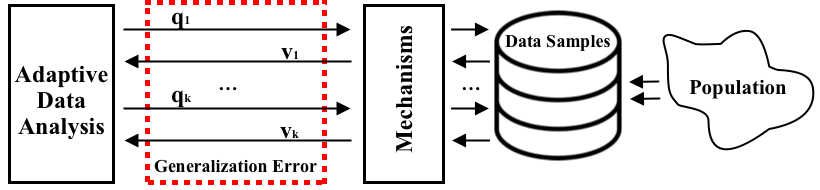
\includegraphics[width=0.7\columnwidth]{figures/data_analysis_model.png}
 \caption{Overview of our Adaptive Data Analysis model.}
 \label{fig:adaptivity-model-overview}
\vspace{-0.5cm}
\end{figure}
This guarantees that the result of the queries generalizes well. 
This approach is described in Figure~\ref{fig:adaptivity-model-overview}, where
I have a population that I am interested in studying, and a dataset containing individual samples from this population. The adaptive data analysis I am interested in running has access to the dataset through queries of some pre-determined family (e.g., statistical or linear queries) mediated by a mechanism. 
This mechanism uses randomization to reduce the generalization error of the queries issued to the data.
This line of work has identified many new algorithmic techniques for ensuring generalization in adaptive data analysis, leading to algorithms with greater statistical power than all previous approaches. 
Common methods proposed by these works include the addition of noise to the result of a query, data splitting, etc. 
Moreover, these works have also identified problematic strategies for adaptive analysis, showing limitations on the statistical power one can hope to achieve. 
Subsequent works have then further extended the methods and techniques in this approach and further extended the theoretical underpinning of this approach, 
e.g.~\cite{dwork2015reusable,dwork2015generalization,BassilyNSSSU16,UllmanSNSS18,FeldmanS17,jung2019new,SteinkeZ20,RogersRSSTW20}.
%

A key development in this line of work is that the best method for ensuring generalization in an adaptive data analysis depends to a large extent on the number of \emph{rounds of adaptivity}, the depth of the chain of queries. 
As an informal example, the program $x \leftarrow \query_1(D);y \leftarrow \query_2(D,x);z \leftarrow \query_3(D,y)$ has three rounds of adaptivity, since $\query_2$ depends on $D$ not only directly because it is one of its input but also via the result of $\query_1$, 
which is also run on $D$, and similarly, $\query_3$ depends on $D$ directly but also via the result of $\query_2$, which in turn depends on the result of $\query_1$. 
The works I discussed above showed that not only does the analysis of the generalization error depend on the number of rounds, 
but knowing the number of rounds allows one to choose methods that lead to the smallest possible generalization error. 

% \mg{Check the following - also the plots need to be on the same scale!}
For example, these works showed that when an adaptive data analysis uses a large number of rounds 
of adaptivity then a low generalization error can be achieved by the mechanism that 
adds Gaussian noise scaled to the number of rounds to each query result.
When instead an adaptive data analysis uses a small number of rounds of adaptivity then a low generalization error can be achieved by using more specialized methods, such as the data splitting mechanism or the reusable holdout technique from~\cite{DworkFHPRR15}.
To better understand this idea, I show in Figure~\ref{fig:generalization_errors} two experiments showcasing these situations. 
More precisely, in Figure~\ref{fig:generalization_errors}(a) shows the results of a real-world analysis
with two rounds of adaptivity. 
This analysis can be seen as a classifier that first runs 500 non-adaptive queries on the first 500 attributes of the data, looking for correlations between the attributes and a label, and then runs one last query which depends on all these correlations. 
Without any mechanism, the generalization error is pretty large, and the lower generalization error is achieved when the data-splitting method is used. 
In Figure~\ref{fig:generalization_errors}(b) shows the results of a specific analysis
with four hundred rounds of adaptivity. 
This analysis can be seen as a classifier that at each step runs an adaptive query based on the result of the previous ones. 
Again, without any mechanism, the generalization error is pretty large, and the lower generalization error is achieved when the Gaussian noise is used. 
{\small
\begin{figure}
\centering
\begin{subfigure}{.48\textwidth}
\begin{centering}
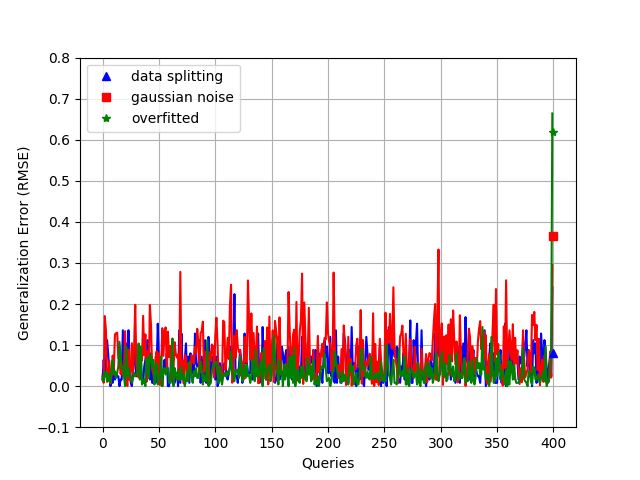
\includegraphics[width=0.9\textwidth]{figures/tworound.png}
\caption{}
\end{centering}
\end{subfigure}
%}
\quad
\begin{subfigure}{.48\textwidth}
\begin{centering}
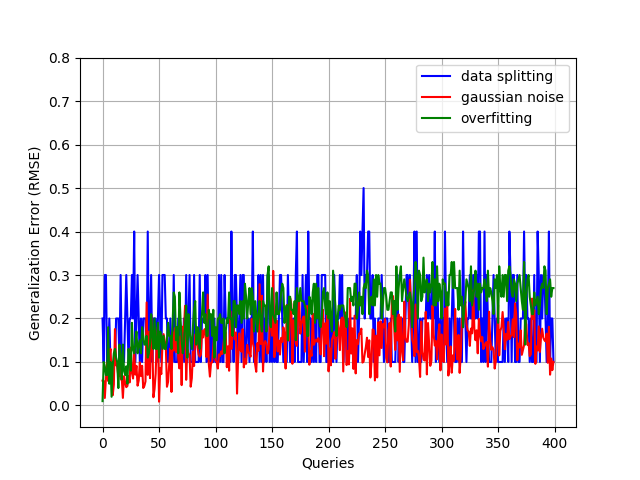
\includegraphics[width=0.9\textwidth]{figures/multipleround.png}
\caption{}
\end{centering}
\end{subfigure}
\vspace{-0.4cm}
 \caption{
 The generalization errors of two adaptive data analysis examples, under different choices of mechanisms.
 (a) Data analysis with adaptivity 2, 
 (b) Data analysis with adaptivity 400. 
}
\label{fig:generalization_errors}
\vspace{-0.5cm}
\end{figure}
}
%gap
This scenario motivates us to explore the design of program analysis techniques that can be used to estimate the number of \emph{rounds of adaptivity} that a program implementing a data analysis can perform. These techniques could be used to help a data analyst in the choice of the mechanism to use,
and they
could ultimately be integrated into a tool for adaptive data analysis such as the \emph{Guess and Check} framework by~\cite{RogersRSSTW20}. 
%
In order to analyze this property, there is mainly three property. 
In this proposal, I will first focus on analyzing 
this adaptivity property for the program is based on solving the three problems specifically as follows.

\paragraph{Challenges of Analyzing Adaptivity}
\label{sec:intro-challenge}
% \subsection{Full-Spectrum Adaptivity Analysis and Methodology}
% \label{subsec:intro-exe}
There are mainly three challenges in order to analyze this adaptivity property, 
and the full-spectrum analysis of this property is 
% In this proposal, I will first focus on analyzing 
% this adaptivity property for the program based on solving 
developed w.r.t. the three challenges accordingly.

\begin{enumerate}
 \item
 \textbf{Adaptive Data Analysis Formalization}

The first challenge is \emph{how to define formally} a model for adaptive data analysis which is general enough to support the methods I discussed above and would permit to formulate the notion of adaptivity these methods use. 
I take the approach of designing a programming framework for submitting queries to some \emph{mechanism} giving access 
to the data mediated by one of the techniques which are mentioned before, 
including the mechanism of adding Gaussian noise, 
the mechanism that randomly selects a subset of the data, 
and the mechanism that uses the reusable holdout technique, etc. 
In this approach, a program models an \emph{analyst} asking a sequence of queries to the mechanism. 
The mechanism runs the queries on the data applying one of the methods discussed above and returns the result to the program. The program can then use this result to decide which query to run next. 
% Overall, I am interested in controlling the generalization of the results of the queries which are returned by the mechanism, by means of adaptivity. 

% \textbf{Methodology}
Motivated by this, I present a while-like language 
named {\tt Query While} language with extensions on query requests in Chapter~\ref{ch:language}.

\item 
\textbf{Adaptivity Formalization}

The second challenge is \emph{how to define the adaptivity of a given program}.
Intuitively, a query $Q$ may depend on another query $P$, if there are two values that $P$ can return which affect in different ways the execution of $Q$. 
For example, as shown in \cite{dwork2015reusable}, and as I did in our example in Figure~\ref{fig:generalization_errors}(a), one can design a machine learning algorithm for constructing a classifier that first computes each feature's correlations with the label via a sequence of queries, and then constructs the classifier based on the correlation values. 
If one feature's correlation changes, the classifier depending on features is also affected. 
This notion of dependency builds on the execution trace as a \emph{causal history}. 
In particular, I am interested in the history or provenance of a query up until this is executed, 
% I am not then concerned about how the result is used --- except for 
simultaneously in tracking whether the result of the query may further cause some other query. 
This is because I'm focusing on the generalization error which could be propagated by queries.
% and not their post-processing. % 

To formalize this intuitive \emph{adaptivity} as a quantitative program property, 
I develop an execution-based analysis in Chapter~\ref{ch:dynamic}.
% \textbf{Methodology}
% % I first consider all the possible evaluations of a program --- I do this by 
% % I use a trace semantics recording the execution history of programs on some given input --- and I create a dependency graph, where the dependency between different variables (query is also assigned to a variable) is explicit and track which variable is associated with a query request. 
% % I then enrich this graph with weights describing the maximal number of times each variable is evaluated in a program evaluation starting with an initial state. The adaptivity is then defined as the length of the walk visiting most query-related variables on this graph. 
% % Through two aspects: the execution-based analysis and static-based program analysis.
% % In the execution-based analysis, I will formalize the intuitive notion of \emph{adaptivity} as a quantitative 
% % property of programs. This analysis is developed 
%  This execution-based analysis is designed in three steps through different methodologies as follows,
%  \begin{enumerate}
%  \item The first step is to analyze the \emph{dependency relation} between every query, 
%  through the methodology of semantic data dependency analysis.
%  %
%  Specifically through a trace semantics recording the execution history of programs on given input,
%  % --- and I create a dependency graph, 
%  the dependency between different variables (query is also assigned to a variable) is explicitly tracked and 
%  analyzed.
% %   and 
% %   which variable is associated with a query request. 
% % I then enrich this graph with weights describing the maximal number of times each variable is evaluated in a program evaluation starting with an initial state. The adaptivity is then defined as the length of the walk visiting most query-related variables on this graph. 
% % In the execution-based analysis, I will formalize the intuitive notion of \emph{adaptivity} as a quantitative 
% % property of programs. This analysis is developed 
% % \\
%  \item The second step is to analyze the \emph{dependency quantity} 
% %  analysis, 
% based on the \emph{dependency relation} above.
% This analysis is developed through the methodology of execution-based reachability bound analysis.
% % \\
%  \item The last step is the intuitive \emph{adaptivity} quantity analysis, 
%  according to the two analysis results above, specifically \emph{dependency relation} and \emph{dependency quantity}.
%  This step 
% %  is developed through 
% gives the formal \emph{adaptivity} definition as the analysis result. \\
%  Specifically, this analysis is developed through creating a dependency graph firstly. 
%  In this graph, the dependency between different variables (query is also assigned to a variable) 
%  is explicit and track which variable is associated with a query request. 
%  This dependency comes from the \emph{dependency relation} from the first step analysis.
%  \\
% Then, I enrich this graph with 
% weights describing the maximal number of times each variable is evaluated in a program evaluation starting with an initial state. 
% This weight comes from the \emph{dependency quantity} from the second step analysis results.
% \\
%  The adaptivity is then defined as the length of the walk visiting most query-related variables on this graph. 
%  \end{enumerate}
\item 
\textbf{Adaptivity Estimation}

The third challenge is \emph{how to estimate the adaptivity of a given program}. 
The adaptive data analysis model I consider and our definition of adaptivity suggest that for this task 
I can use a program analysis that is based on some form of dependency analysis.
 This analysis needs to take into consideration:
1) the fact that, in general, a query $Q$ is not a monolithic block but rather it may depend, through the use of variables and values, on other parts of the program. 
Hence, it needs to consider some form of data flow analysis. 
2) the fact that, in general, the decision on whether to run a query or not may depend on some other value. Hence, 
 it needs to consider some form of control flow analysis.
3) the fact that. in general, I am not only interested in whether there is a dependency or not, but in the length of the chain of dependencies. 
Hence, it needs to consider some quantitative information about the program dependencies. % {A quick example is that: I store the result of query $Q_1$ in variable $x$ and use variable $y$ to record the result of query $Q_2$. I want to construct the third query $Q_3$ which relies on the value stored in $x$, let us say, $Q_3$ will ask for the sum of the first column of a table if $x$ is positive and the sum of the second column otherwise. In this situation, I need data flow analysis. On the other hand, if I need the value of $y$ to help us decide whether I should ask $Q_3$, for example, I ask the third query if $y$ is odd, and do not ask if $y$ is even. Naturally, to be able to handle this case, control flow analysis comes into play. Formally speaking, }

To address these considerations and be able to estimate a sound upper bound on the adaptivity of a program, 
I develop a static program analysis in Chapter~\ref{ch:static}, named {\THESYSTEM}.
%%%%% To reason about%
\end{enumerate}
% \\
%
\section{Execution-Based Program Analysis}
\label{sec:intro-exe}
% \begin{enumerate}
%  \item
%  \textbf{Adaptive Data Analysis Formalization}
% The first challenge is \emph{how to define formally} a model for adaptive data analysis which is general enough to support the methods I discussed above and would permit to formulate the notion of adaptivity these methods use. 
% I take the approach of designing a programming framework for submitting queries to some \emph{mechanism} giving access to the data mediated by one of the techniques I mentioned before, e.g., adding Gaussian noise, randomly selecting a subset of the data, using the reusable holdout technique, etc. 
% In this approach, a program models an \emph{analyst} asking a sequence of queries to the mechanism. The mechanism runs the queries on the data applying one of the methods discussed above and returns the result to the program. The program can then use this result to decide which query to run next. 
% % Overall, I'm interested in controlling the generalization of the results of the queries which are returned by the mechanism, by means of adaptivity. 
% \item 
\paragraph{Research Goal - Adaptivity Formalization}
Targeting on the second challenge
% --\textbf{Adaptivity Formalization}--
for analyzing the adaptivity, 
the research goal is to develop analysis method which can
% The second challenge is 
\emph{define} the intuitive \emph{adaptivity} rounds for a given data analysis program formally and accurately.
% Intuitively, a query $Q$ may depend on another query $P$, if there are two values that $P$ can return which affect in different ways the execution of $Q$. 
% For example, as shown in \cite{dwork2015reusable}, and as I did in our example in Figure~\ref{fig:generalization_errors}(a), one can design a machine learning algorithm for constructing a classifier that first computes each feature's correlations with the label via a sequence of queries, and then constructs the classifier based on the correlation values. 
% If one feature's correlation changes, the classifier depending on features is also affected. 
The intuition behind this \emph{adaptivity} quantity relies on the dependency between the query requests 
executed in the program, and their dependency depth. 
% This notion of dependency builds on the execution trace as a \emph{causal history}. 
Following this intuition, we need to formally define whether there is dependency between query requests during the program
execution.
%
% And the 
There are different methodologies can be used to formalize the dependency between two query requests, such as the 
dynamic analysis, execution-based analysis, static analysis, etc.
%
In order to capture the dependency (also the intuitive \emph{adaptivity}) in the most precise way,
I design the execution-based program analysis method.
%
% In order to define it in 
% The most precise way to define this dependency is by observing the actual evaluation of these query requests during the 
% program execution.
This execution-based program analysis method is precise in formalizing the dependency relation
%  between query requests,
and the intuitive \emph{adaptivity} because it is
% In particular, I'm interested in the history or provenance of a query up until this is executed, I'm not then concerned about how the result is used --- except for tracking whether the result of the query may further cause some other query. 
% Based on this, I design the adaptivity formalization method through the execution-based program analysis techniques.
% These execution-based analysis techniques are 
based on observing the actual evaluation of these query requests during the 
program execution. This is consistent with the intuition of query requests dependency and their dependency depth,
as well as the intuitive
\emph{adaptivity}.
% This is because I focus on the generalization error of queries and not their post-processing. % 
\paragraph{Limitations of Existing Execution-Based Program Analysis Techniques}
There are many techniques in the execution-based analysis areas, such are the program simulation, 
semantics analysis, abstract interpretation, etc., which are widely used in dependency analysis. 
However, it is not straightforward that how to apply them into analyzing and formalizing the \emph{adaptivity}
for adaptive data analysis program.
There are following three limitations among existing execution-based analysis techniques.
\begin{enumerate}
\item The state-of-art execution-based dependency relation analysis techniques don't
consider both control influence and value influence. However, both of these
two influences are included by the intuitive query dependency 
in adaptive data analysis programs.
%  require
\item The existing execution-based data dependency analysis area, there isn't any technique taking into account
the dependency depth. However, this dependency depth is the key quantity in formalizing the intuitive \emph{adaptivity}.
\item The intuitive \emph{adaptivity} doesn't accumulate linearly through the dependency relation and 
dependency depth. There is only very limited works related to this non-linear quantity property analysis.
This requires us to design new analysis techniques in order to formalize this quantity precisely.
% here isn't any research combining the two information. No need to mention the adaptivity analysis.
\end{enumerate}
%
\paragraph{Methodology Overview}
% To formalize this intuition as a quantitative program property, 
% in Chapter~\ref{ch:dynamic} I develop an execution-based analysis
% % I first consider all the possible evaluations of a program --- I do this by 
% % I use a trace semantics recording the execution history of programs on some given input --- and I create a dependency graph, where the dependency between different variables (query is also assigned to a variable) is explicit and track which variable is associated with a query request. 
% % I then enrich this graph with weights describing the maximal number of times each variable is evaluated in a program evaluation starting with an initial state. The adaptivity is then defined as the length of the walk visiting most query-related variables on this graph. 
% % Through two aspects: the execution-based analysis and static-based program analysis.
% % In the execution-based analysis, I will formalize the intuitive notion of \emph{adaptivity} as a quantitative 
% % property of programs. This analysis is developed 
%  in three steps through different methodologies in each step as follows,
 To formalize this intuitive \emph{adaptivity} as a quantitative program property, 
I develop an execution-based analysis in Chapter~\ref{ch:dynamic}.
% I first consider all the possible evaluations of a program --- I do this by 
% I use a trace semantics recording the execution history of programs on some given input --- and I create a dependency graph, where the dependency between different variables (query is also assigned to a variable) is explicit and track which variable is associated with a query request. 
% I then enrich this graph with weights describing the maximal number of times each variable is evaluated in a program evaluation starting with an initial state. The adaptivity is then defined as the length of the walk visiting most query-related variables on this graph. 
% Through two aspects: the execution-based analysis and static-based program analysis.
% In the execution-based analysis, I will formalize the intuitive notion of \emph{adaptivity} as a quantitative 
% property of programs. This analysis is developed 
 This execution-based analysis is designed in three steps through different methodologies as follows,
%  \begin{enumerate}
%  \item The dependency relation between every query, through the methodology of semantic data dependency analysis.
%  \\
%  Specifically through a trace semantics recording the execution history of programs on some given input
%  % --- and I create a dependency graph, 
%  the dependency between different variables (query is also assigned to a variable) is explicit and track which variable is associated with a query request. 
% % I then enrich this graph with weights describing the maximal number of times each variable is evaluated in a program evaluation starting with an initial state. The adaptivity is then defined as the length of the walk visiting most query-related variables on this graph. 
% % In the execution-based analysis, I will formalize the intuitive notion of \emph{adaptivity} as a quantitative 
% % property of programs. This analysis is developed 
% % \\
%  \item The dependency quantity analysis, through the methodology of execution-based data reachability, bound analysis.
% % \\
%  \item The adaptivity quantity analysis, based on the two analysis results above, gives the formal \emph{adaptivity} model 
%  for program.
%  \\
%  Specifically, I create a dependency graph, where the dependency between different variables (query is also assigned to a variable) is explicit and track which variable is associated with a query request. 
%  I then enrich this graph with weights describing the maximal number of times each variable is evaluated in a program evaluation starting with an initial state. 
%  The adaptivity is then defined as the length of the walk visiting most query-related variables on this graph. 
%  \end{enumerate}
\begin{enumerate}
   \item First step is to analyze the \emph{dependency relation} between every query, 
   through the methodology of semantic data dependency analysis.
   %
   Specifically through a trace semantics recording the execution history of programs on given input,
   % --- and I create a dependency graph, 
   the dependency between different variables (query is also assigned to a variable) is explicitly tracked and 
   analyzed. This is presented in Section~\ref{sec:dynamic-datadep}.
  %   and 
  %   which variable is associated with a query request. 
  % I then enrich this graph with weights describing the maximal number of times each variable is evaluated in a program evaluation starting with an initial state. The adaptivity is then defined as the length of the walk visiting most query-related variables on this graph. 
  % In the execution-based analysis, I will formalize the intuitive notion of \emph{adaptivity} as a quantitative 
  % property of programs. This analysis is developed 
  % \\
   \item The second step in Section~\ref{sec:dynamic-reachability} is to analyze the \emph{dependency quantity} 
  %  analysis, 
  based on the \emph{dependency relation} above.
  This analysis is developed through the methodology of execution-based reachability bound analysis.
  % \\
   % \item The last step in Section~\ref{sec:dynamic-adapt}  is the intuitive \emph{adaptivity} quantity analysis, 
   % according to the two analysis results above, specifically \emph{dependency relation} and \emph{dependency quantity}.
   % This analysis is developed through the formal \emph{adaptivity} definition. \\
   % Specifically, I create a dependency graph, where the dependency between different variables (query is also assigned to a variable) is explicit and track which variable is associated with a query request. 
   % I then enrich this graph with weights describing the maximal number of times each variable is evaluated in a program evaluation starting with an initial state. 
   % The adaptivity is then defined as the length of the walk visiting most query-related variables on this graph. 
   \item The last step is the intuitive \emph{adaptivity} quantity analysis, 
   according to the two analysis results above, specifically \emph{dependency relation} and \emph{dependency quantity}.
   This step 
  %  is developed through 
  gives the formal \emph{adaptivity} definition as the analysis result. 
  \\
  Specifically, this analysis is developed through creating a dependency graph firstly. 
  In this graph, the dependency between different variables (query is also assigned to a variable) 
  is explicit and track which variable is associated with a query request. 
  This dependency comes from the \emph{dependency relation} from the first step analysis.
  \\
 Then, I enrich this graph with 
 weights describing the maximal number of times each variable is evaluated in a program evaluation starting with an initial state. 
 This weight comes from the \emph{dependency quantity} from the second step analysis results.
 \\
  The adaptivity is then defined as the length of the walk visiting most query-related variables on this graph. 
      \end{enumerate}
   % \item 
\section{Static Program Analysis}
\label{sec:intro-static}
% \paragraph{Limitations of Existing Execution-Based Program Analysis Techniques}
%
Though we have the intuitive \emph{Adaptivity} formally and precisely defined through the execution-based program analysis,
it is still not useful enough for programmers.
The weakness of the execution-based analysis comes from its in-efficiency.
It can only give the \emph{Adaptivity} number
after the program is executed multiple times.
When the query requests, the multiple executions consume large amount of computation and communication resources.
This requires us to develop an efficient analysis method, 
which can provide the programmers with the \emph{Adaptivity} quantity.
Because the static program analysis techniques usually don't require the execution of the program,
they are more efficient than the execution-based analysis.
Motivated by this, we develop a static program analysis framework, named {\THESYSTEM}.
% the  through static-based 
% program analysis techniques.
% % In order to provide the programmers with the useful information in an efficiency way,
% I develop a static program analysis
% to estimate this adaptivity quantity efficiently.
% % , also without lose the usefulness of the information. 
% Through
\paragraph{Research Goal - Adaptivity Estimation}
Targeting on the third challenge
% --\textbf{Adaptivity Formalization}--
for estimating the adaptivity, 
the major research goal is to develop analysis method which can
% The second challenge is 
% give a sound and accurate \emph{upper bound} for the 
provide the programmers with the \emph{adaptivity} quantity
soundly, accurately and
efficiently
% defined 
through static program analysis.
%  for a given data analysis program.
% Intuitively, a query $Q$ may depend on another query $P$, if there are two values that $P$ can return which affect in different ways the execution of $Q$. 
% For example, as shown in \cite{dwork2015reusable}, and as I did in our example in Figure~\ref{fig:generalization_errors}(a), one can design a machine learning algorithm for constructing a classifier that first computes each feature's correlations with the label via a sequence of queries, and then constructs the classifier based on the correlation values. 
% If one feature's correlation changes, the classifier depending on features is also affected. 
% The adaptive data analysis model I consider and our definition of adaptivity suggest that for this task I can use a program analysis that is based on some form of dependency analysis. This analysis needs to take into consideration:
There are three sub-research goals in estimating \emph{adaptivity} statically.
Each goal aims to resolve a fact introduced in the \textbf{Adaptivity Estimation} challenge in Section~\ref{sec:intro-motivation}.
\\
subgoal-1) Designing data flow analysis algorithm, aims to estimate whether a query may dependent on the other queries. 
This analysis needs to consider the monolithic blocks of program, through the use of variables and values, on other parts of the program.
% the fact that, in general, a query $Q$ is not a monolithic block but rather it may depend, 
% through the use of variables and values, on other parts of the program. 
% Hence, it needs to consider some form of data flow analysis. 
\\
subgoal-2) Integrating the control flow analysis techniques into the static analysis,
 aims to 
capture the query dependency soundly
%  in the case
%   fact that, in general, the decision on 
% where the dependent query might not be executed under the 
under the control influence.
%  of the first query. 
% Hence, 
%  it needs to consider some form of control flow analysis.
 \\
subgoal-3) Combining the reachability bound analysis techniques into the static analysis,
%   I'm not only interested in whether there is a dependency or not, but in the length of the chain of dependencies. 
% Hence, it needs to consider some 
aims to estimate
%  the quantitative information on the query requests dependencies. 
the dependency depth for query requests.
% {A quick example is that: I store the result of query $Q_1$ in variable $x$ and use variable $y$ to record the result of query $Q_2$. I want to construct the third query $Q_3$ which relies on the value stored in $x$, let us say, $Q_3$ will ask for the sum of the first column of a table if $x$ is positive and the sum of the second column otherwise. In this situation, I need data flow analysis. On the other hand, if I need the value of $y$ to help us decide whether I should ask $Q_3$, for example, I ask the third query if $y$ is odd, and do not ask if $y$ is even. Naturally, to be able to handle this case, control flow analysis comes into play. Formally speaking, }
\paragraph{Limitations of Existing Program Analysis Techniques}
There are many execution-based program analysis techniques, which are widely used in  dependency analysis. 
However, it is not straightforward when applying to adaptivity analysis.
\begin{enumerate}
\item there isn't static dependency analysis techniques consider both control influence and value influence so far
\item existing static complexity analysis techniques cannot give accurate reachability times on programs 
every execution location path sensitively.
\item there isn't any research or static analysis considering both the dependency analysis
and the complexity. No need to mention the adaptivity analysis.
\end{enumerate}

\paragraph{Methodology}
To address these considerations and be able to estimate a sound upper bound on the adaptivity of a program, 
I develop a static program adaptivity analysis framework, named {\THESYSTEM} in Chapter~\ref{ch:static}.
%  which 
% {\THESYSTEM} combines data flow and control flow analysis with reachability bound analysis~\cite{GulwaniZ10}. 
% This new program analysis gives tighter bounds on the adaptivity of a program than the ones one would achieve by directly using the data and control flow analyses or the ones that one would achieve by directly using reachability bound analysis techniques alone. Specifically as follows in the same 3 aspects as the execution-based analysis 
% while through static program analysis techniques, a sound estimated result will be given in each aspect as follows.
This analysis combines data flow and control flow analysis with reachability bound analysis.
% ~\cite{GulwaniZ10}. 
This new program analysis gives tighter bounds on the adaptivity of a program than the ones one would achieve 
by directly using the data and control flow analyses or the ones that one would achieve 
by directly using reachability bound analysis techniques alone. 
% Specifically as follows in the same 
It is developed in 3 aspects similar to the execution-based adaptivity analysis 
while through static program analysis techniques. 
A sound estimated result is given in each part, which is summarized as follows.
\begin{enumerate}
% \item The data dependency relation analysis through the static data flow analysis technique.
% \item The dependency quantity analysis through the static program reachability bound analysis techniques.
% \item The program adaptivity estimation, through newly designed algorithms based on the results estimated above, 
% computing the adaptivity upper bound soundly 
% and accurately.
\item The {\THESYSTEM} analyzes the data \emph{dependency relation} through the static data flow analysis technique in Section~\ref{sec:alg_weightedgegen}.
This analysis corresponds to the first step in execution-based adaptivity analysis. 
The estimated result produced from 
this step is proved as a sound upper bound for the \emph{dependency relation} from execution-based analysis.
\item 
% Still , 
Corresponding to the second step in execution-based adaptivity analysis, the \emph{dependency quantity} 
is estimated by {\THESYSTEM} through the static program reachability bound analysis techniques, in Section~\ref{sec:alg_weightedgegen}.
% This analysis corresponds to the second step in execution-based adaptivity analysis. 
The estimated result produced from 
this step is proved as a sound upper bound for the \emph{dependency quantity} from execution-based analysis as well.
\item 
% The program  estimation, 
% In 
The static program adaptivity analysis in this step
% , specifically estimating 
estimates the \emph{adaptivity} formalized in the third step of execution-based analysis in Section~\ref{sec:static-adapt}.
%  is presented in Section~\ref{sec:static-reachability}.
% the program adaptivity estimation, 
According to the third step of execution-based adaptivity analysis, 
{\THESYSTEM} in this step also constructs a program-based dependence graph for approximating the execution-based dependency graph.
%  in Section~\ref{sec:dynamic-adapt}.
Then, based on this graph, {\THESYSTEM} 
% I design an algorithm
%  based on the results estimated above, 
% computing 
computes the adaptivity upper bound soundly 
and accurately through a newly designed algorithm.
\end{enumerate}

\subsection{\todo{PSRB: integrated this into the Section~\ref{sec:intro-static} or separately}}
Given the limitation of existing reachability bound analysis techniques, I designed a path-sensitive reachability bound 
analysis algorithm

Based on the implementation and experimental results of the basic full-spectrum analysis,
% $\THESYSTEM$,
I 
% also focus on the two further features can be 
extend it in Section~\ref{ch:improved} in following 3 aspects.
% \begin{enumerate}
%  \item The precision of formalizing the intuitive \emph{adaptivity} 
% %  in the formal  model 
% through the execution-based program analysis.

% \item In static program analysis, I will give a tighter estimated upper bound on dependency quantity through 
% path sensitive reachability bound analysis techniques. 

% % \item In the third step of static program analysis, I will improve the accuracy of the adaptivity computation algorithm,
% % compute a tighter adaptivity upper bound as well.
% \end{enumerate}
\begin{enumerate}
   \item The {\tt Query While} Language is extended in Section~\ref{sec:refine-exe-language} with inter-procedure call.
   \item In the execution-based \emph{adaptivity} analysis part,
   the precision of formalizing the intuitive \emph{adaptivity} is improved, with extension on the
%  in the formal  model 
% in the meantime extend this analysis with 
inter-procedure call in Section~\ref{sec:refine-exe}.
\item The static program \emph{adaptivity} analysis is extended inter-procedure call as well, 
and improved by
giving a tighter estimated upper bound on \emph{adaptivity} in Section~\ref{sec:refine-static}.
%  give a tighter estimated upper bound 
Especially in order to improve the accuracy of the estimated result, a
% I improve the accuracy of the static \emph{dependency quantity} analysis in the second step through 
% designing a
path sensitive reachability bound analysis algorithm is designed in Section~\ref{sec:refine-static-psreachability}.
Based on this newly designed algorithm,
I improve the accuracy of the static \emph{dependency quantity} analysis in the second step 
is improved, and a tighter upper bound on \emph{adaptivity} is computed correspondingly.
% \item In the third step of static program analysis, I will improve the accuracy of the adaptivity computation algorithm,
% compute a tighter adaptivity upper bound as well.
\end{enumerate}

%%%%% To reason about%
\section{Analysis Framework Overview}
Figure~\ref{fig:structure} is the overview of this full-spectrum program adaptivity analysis.
% There are mainly three parts, each targeting on a challenge above.
It is composed of three parts, each targeting on a challenge above.
The fundamental part is the {\tt Query While} language designed for formalizing the 
adaptive data analysis. Building on this, 
the execution-based adaptivity analysis (formalization)
and the static program analysis for approximating the upper bound of the 
adaptivity are the two major analysis parts of this full-spectrum adaptivity analysis.
\begin{figure}
   \centering   
   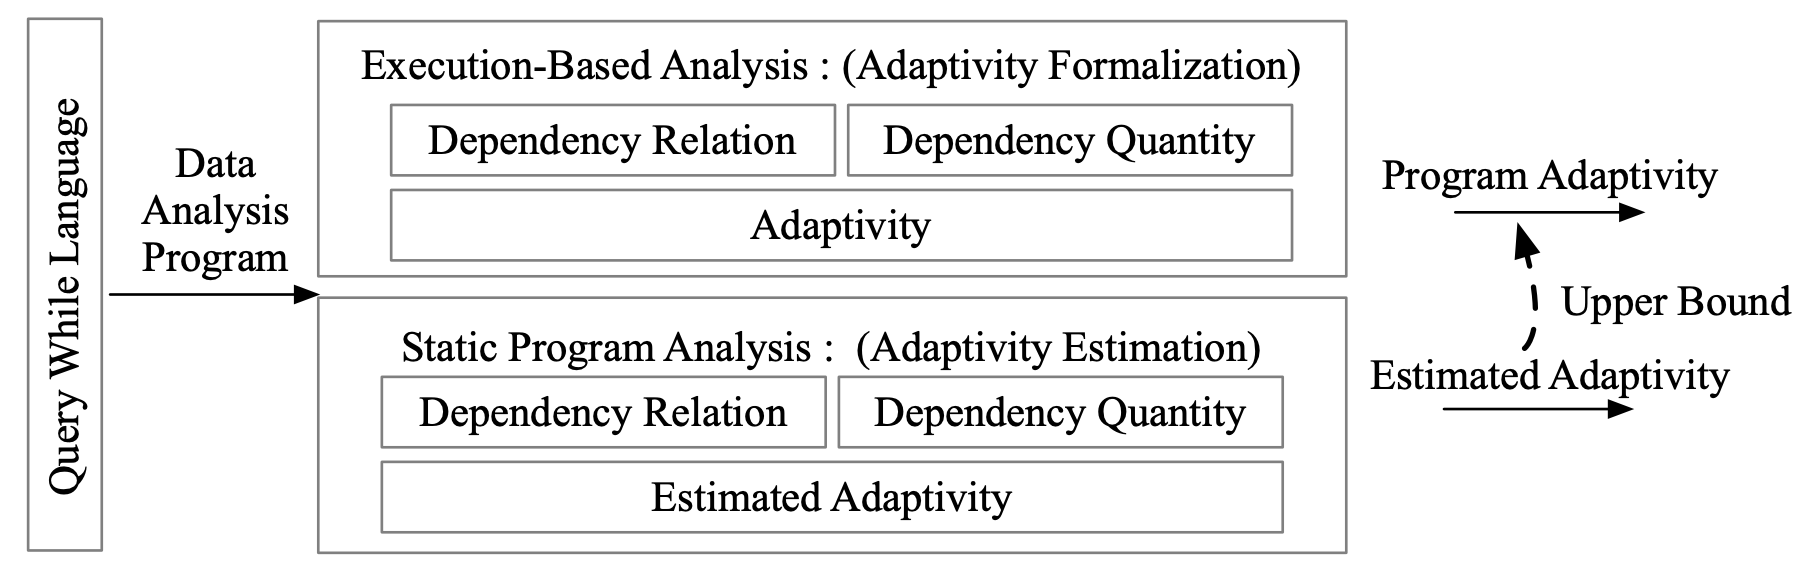
\includegraphics[width=1.0\textwidth]{figures/overview.png}
  \caption{High level architecture of the Program Analysis Framework for Adaptivity Analysis}
   \label{fig:structure}
\end{figure}
% \end{enumerate}% \\

% \subsection{Further Works}
% \subsubsection{Towards Accurate Full-Spectrum Adaptivity Analysis}
% \label{sec:intro-improve}


% \\
\section{Future Works}
\label{sec:intro-cfl}
\paragraph{Program Resource Cost Analysis}
\label{sec:intro-cost}
% Then, motivated by the two following aspects, I'm interested in improving the accuracy of the program's general resource cost analysis
% by generalizing this \emph{adaptivity} analysis framework.
Moving towards the area of general program resource cost analysis,
% Then, motivated by the two following aspects, 
there are two interesting observations as follows.
% I'm interested 
These two observations motivated me in 
% improving the accuracy of the program's general resource cost analysis
improving the accuracy of the program's general resource cost analysis
by generalizing this full-spectrum \emph{adaptivity} analysis.
\begin{itemize}
 \item Firstly, in a traditional program's resource cost analysis,
 There are two categories of program cost analysis, type-system based and data-flow/control-flow analysis based. 
 In the type-system design-based works, they \cite{GustafssonEL05} and \cite{hoffmann_jost_2022}, explicit abstraction or data structure de-allocation in order to save or reduce the cost.
 
 Both of the
 works in these two areas fail to recognize the case where program resource consumption is decreased implicitly.
 \item The resource consumption during the program 
 execution increases and particularly decreases implicitly in the same way as the program's adaptivity. 
 This is explained in detail through an example in Section~\ref*{sec:generalcost-backgroung}.
\end{itemize}
% F
% Then, through two observations,
% that 
% firstly, traditional program's resource cost analysis failed to consider the case where the program's cost could decrease 
% implicitly, and 
% % when there isn't a dependency relation between variables.
% the resource consumption during the program 
% execution increases and particularly decreases implicitly in the same way as the program's adaptivity, 
% % Specifically, in line 5 
% % where the list is re-written and the heap consumption is decreased implicitly. 
% % This implicit decrease 
% % of the cost works exactly the same as the program's adaptivity decrease.
% I'm interested in improving the accuracy of the program's general resource cost analysis
% by generalizing my \emph{adaptivity} analysis framework.
 % onto the program's resource cost analysis. 
 % Use this framework,
 Based on the observations above, in Chapter~\ref{ch:generalization},
%  Based on the observations above, and through the generalized \emph{adaptivity} analysis framework.
%  I will give
%  a more accurate resource cost estimation by taking the program's implicit resource cost into consideration, compared 
%  to the worst-case cost analysis in the traditional way.
 I develop
 an accurate program general resource cost analysis framework through generalizing my full-spectrum \emph{adaptivity} analysis.
 This framework can give more accurate cost bound than traditional worst-case resource cost estimation methods,
 by taking the program's implicit resource cost into consideration.
% F
% Then, through two observations,
%    that 
%    firstly, traditional program's resource cost analysis they failed to consider the case where the program's cost could decrease 
%    implicitly, and 
%    % when there isn't a dependency relation between variables.
%    the resource consumption during the program 
%    execution increases and particularly decreases implicitly in the same way as the program's adaptivity, 
%    % Specifically, in line 5 
%    % where the list is re-written and the heap consumption is decreased implicitly. 
%    % This implicit decrease 
%    % of the cost works exactly the same as program's adaptivity decrease.
%    I'm interested in improving the accuracy of program's general resource cost analysis
%    by generalizing my \emph{adaptivity} analysis framework.
   %  onto the program's resource cost analysis. 
   % Use this framework,
   % Based on the observations above, and through the generalized \emph{adaptivity} analysis framework.
   % I will give
   % a more accurate resource cost estimation by taking the program's implicit resource cost into consideration, comparing 
   % to the worst case cost analysis in traditional way.

%    \section{Towards Solving the CFL-Reachability Problem}
% Finally, based on the study on traditional way of performing data flow and control analysis,
% I identify the similarity between the traditional way of performing data flow and control analysis, and the 
%    adaptivity analysis.  
%    Specifically I identify the similarity between 
%    solving the feasible path problem in the analysis by reducing to CFL-reachability problems,
%    and the way of computing the adaptivity in my static analysis framework.
%    Motivated by this observation, 
%    % I'm insterested
%    % the, There are similarity between
%    % solving the data flow problem by reducing to CFL-reachability problem,
%    % resource analysis through reducing to CFL-reachability problem, 
%    I'm interested in showing that
%    CFL-reachability problems can be solved by reducing it into my adaptivity analysis framework.

\paragraph*{Solving the CFL Reachability Problem}
Still in the area of general program resource cost analysis,
the traditional methodology of performing data flow and control analysis and 
computing the program resource cost is
% Finally, based on the study on the traditional way of performing data flow and control analysis,
to reduce the analysis problem into the CFL-reachability problems.
% Finally, based on the study on the traditional way of performing data flow and control analysis,
According to this, 
I identify x
% the similarity between the traditional way of performing data flow and control analysis and the 
the similarities between the traditional way of estimating the program resource cost and 
the adaptivity.
%  Specifically, I identify the similarity between 
%  solving the feasible path problem in the analysis by reducing 
Specifically, there are similarities between solving the CFL-reachability problems they reduced to,
%  CFL-reachability problems,
 and the way of computing the adaptivity in 
%  my static analysis framework.
the third step of $\THESYSTEM$.
 Motivated by this, 
 % I'm Interested
 % the, There are similarities between
 % solving the data flow problem by reducing to CFL-reachability problem,
 % resource analysis through reducing to CFL-reachability problem, 
 I'm interested in showing that
 CFL-reachability problems can be solved by reducing to my adaptivity analysis framework.
In Chapter~\ref{ch:furthers}, I started this work and proposed plans on developing this work in the furture.


%%%%% To reason about
% \section{Methodology}
% We use static analysis techniques to reason about the two main quantitative properties studied in this dissertation: 
% the adaptivity of adaptive data analysis programs,
% the reachability bound of while loop programs. 

% \subsection{Abstract Interpretation}

% \subsection{Dependency Graph}
% Another quantitative property we study is the adaptivity of adaptive data analysis programs. 
% {The adaptivity is defined to be the length of the longest chain of queries of the program in which one query may rely 
% on its previous queries in the same chain. 
% The adaptivity of a data analysis program is quite different from the relative cost of the two programs. To reason about cost, we can simply sum the costs of sub-programs to get the upper bound of the cost. However, the adaptivity of each sub-program of the target program does not help much in finding the adaptivity. To use a type and effect system to reason about adaptivity, this system should be able to express certain dependencies.
% % Of course, we can sum them but then the result becomes imprecise. For this reason, we think the type and effect system is not the good direction to reason about the adaptivity of a data analysis program since it is tricky for the effect to carry information such as one query may depend on the other one. 
% We expect adaptivity can also be reasoned about by type and effect systems but in this work, we choose to use a dependency graph to reason about adaptivity.}

% {There are two challenges to reason about adaptivity: what will a formal definition of the adaptivity of a data analysis program look like, and how to reason about the adaptivity. 
% In our work, the first challenge is solved by a query-based dependency graph generated along with the evaluation of the program. 
% Our trace-based operational semantics can generate the trace which tracks the queries asked in the evaluation of the program. 
% The query-based dependency graph is constructed based on the queries in the trace. Every node of the graph represents a unique query asked in the program, and the directed edge between two nodes, identifying one query (one node) may depend on the other one. 
% The adaptivity is then formally defined as the length of the longest path in the query-based dependency graph.}
% {The second challenge is how to estimate the adaptivity of a data analysis program we have just defined. 
% In order to upper bound the length of the longest path in the query-based dependency graph, we want to find a path in a dependency graph as well such that the path contains all the queries in that longest path in the query-based dependency graph. 
% We develop an algorithm to build a variable-based dependency graph, in which every node represents the unique variable that is assigned in one assignment statement of the program. 
% The direct edge between two nodes reflects both the data dependency and control flow dependency between variables. Also, we add the unit weight to the node whose variable is associated with a query result. Then the upper bound on the adaptivity of the data analysis program is estimated by the weight of the path with the highest weights in the variable-based dependency graph.}

% {To summarize, we use two dependency graphs for reasoning about the adaptivity of a data analysis program: 
% one query-based dependency graph to define the adaptivity, and one weighted variable-based dependency graph to estimate an upper bound on the adaptivity. }

\section{Contributions and Outline}
\label{sec:intro-outline}
\paragraph{Contributions}
This dissertation has the following contributions.
\begin{enumerate}
   \item A programming framework for adaptive data analyses where the program represents an analyst that can query a generalization-preserving mechanism mediating the access to some data. 
   % \item A trace-based operational semantics for the loop language, specific to dependency between queries.
   \item 
   % {A formal definition of the notion of adaptivity under the analyst-mechanism model. This definition is built on a query-based dependency graph built out of all the possible program execution traces.}
   A formal definition of the notion of adaptivity under the analyst-mechanism model. 
   This definition is built on a variable-based dependency graph that is constructed using sets of program execution traces.
   % \item A transformation between the {\tt Loop} language and the ssa language, with the soundness of the transformation.
   \item 
   % A program analysis algorithm {\THESYSTEM} which provides an upper bound on the adaptivity via a variable-based dependency graph.
   A static program analysis algorithm {\THESYSTEM} combining data flow, control flow and  reachability bound analysis in order to provide tight bounds on the adaptivity of a program. 
   %
   \item A soundness proof of the program analysis showing that the adaptivity estimated by {\THESYSTEM} bounds the true adaptivity of the program. 
   \item An implementation of {\THESYSTEM} and an experimental evaluation the bounds this implementation provides on several examples.
   \item A path-sensitive program reachability bound analysis algorithm designed for program with application beyond adaptivity analysis
    with implementation.
   % \item An improved formal adaptivity model and {\THESYSTEM} with implementation.
   %  expected to be done before the final defense.
   \item An accurate full-spectrum program resource cost analysis, 
   generalized from {\THESYSTEM} with implementation.
   % The analysis framework design is expected to be done with the implementation start off before the final defense.
      % To the best of our knowledge, it is the first work that statically estimates adaptivity to help design adaptive data analysis algorithms.  
\end{enumerate}
%
\paragraph*{Outline}
This dissertation includes following parts. 
\begin{enumerate}
\item A while-like language extended with query request feature, named {\tt Query While} Language, 
used to implement 
the adaptive data analysis in Chapter~\ref{ch:language}.
\item A formal adaptivity model through execution-based adaptivity analysis in Chapter~\ref{ch:dynamic}.
\item A static program analysis algorithm, named {\THESYSTEM} through static adaptivity analysis in Chapter~\ref{ch:static}.
\item An extended full-spectrum program adaptivity analysis in Chapter~\ref{ch:improved}.
\item An accurate full-spectrum program resource cost analysis, 
generalized from {\THESYSTEM} with implementation in Chapter~\ref{ch:generalization}.
\item Proposed future works for solving the CFL-reachability problem via reduction into the {\THESYSTEM} framework in
Chapter~\ref{ch:furthers},
expected to be started off before final defense and developing further after.
\end{enumerate}



\paragraph{Previous Published Material}
The contents of this dissertation are partly based on the work and writing in the following papers.

% The work of{\ADAPTSYSTEM} is still under preparation.


